% consensus-obj-rw.tex

\documentclass{standalone}

\usepackage{tikz}
\usetikzlibrary{shapes, positioning, arrows.meta, backgrounds, fit}

\begin{document}
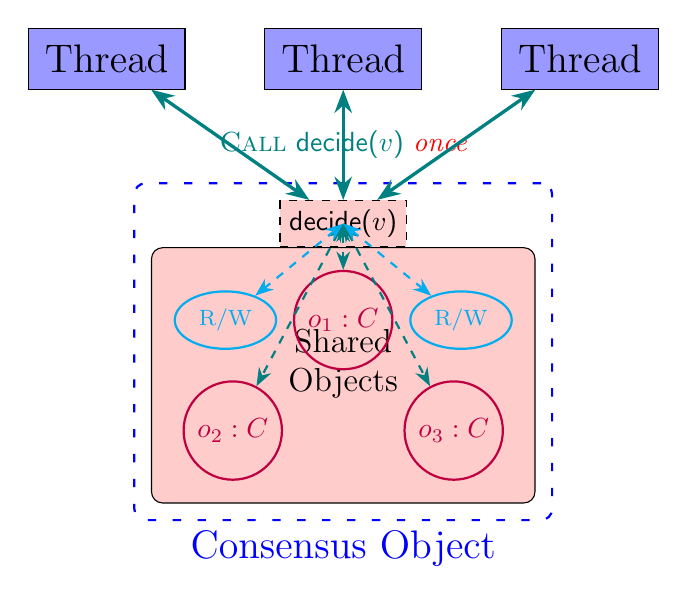
\begin{tikzpicture}[thread/.style = {draw, rectangle, fill = blue!40, font = \Large, inner sep = 6pt},
    call/.style = {>=Stealth, <->, very thick, teal},
    incall/.style = {>=Stealth, <->, thick, dashed, teal},
    obj/.style = {draw, circle, thick, purple, minimum size = 5pt},
    rw/.style = {draw, ellipse, thick, cyan, font = \footnotesize},]
  \node (obj1) [obj] {$o_1: C$};
  \node (obj2) [obj, below left = 0.50cm and 0.50cm of obj1] {$o_2: C$};
  \node (obj3) [obj, below right = 0.50cm and 0.50cm of obj1] {$o_3: C$};

  \node (rw1) [rw, left = 0.20cm of obj1] {R/W};
  \node (rw2) [rw, right = 0.20cm of obj1] {R/W};

  \begin{pgfonlayer}{background}
    \node (so) [draw, rectangle, rounded corners, fit = (obj1) (obj2) (obj3) (rw1) (rw2),
	  font = \large, fill = red!20, align = center, inner sep = 8pt] {Shared \\ Objects};
  \end{pgfonlayer}
  \node (decide) [draw, rectangle, above = 0.0cm of so, dashed, fill = red!20] {\textsf{decide($v$)}};

  \node (tm) [thread, above = 2.0cm of so] {Thread};
  \node (tl) [thread, left = of tm] {Thread};
  \node (tr) [thread, right = of tm] {Thread};

  \draw [call] (tm) to node [] {\textsf{\textsc{Call} decide($v$)} \textcolor{red}{\it once}} (decide);
  \draw [call] (tl) to (decide);
  \draw [call] (tr) to (decide);

  \draw [incall] (decide.center) to (obj1);
  \draw [incall] (decide.center) to (obj2);
  \draw [incall] (decide.center) to (obj3);
  \draw [incall, cyan] (decide.center) to (rw1);
  \draw [incall, cyan] (decide.center) to (rw2);
  
  \begin{pgfonlayer}{background}
    \node (consensus-obj) [draw, thick, blue, rectangle, rounded corners, loosely dashed, fit = (so) (decide), inner sep = 6pt,
	label = {[font = \Large, align = center, blue]-90:{Consensus Object}}] {};
  \end{pgfonlayer}
\end{tikzpicture}
\end{document}
